% Provenance (never printed): cycle 4 SVT/physique, "La planete Terre,
% l'environnement": the atmosphere, its structure and its layers, pressure
% and altitude, the ozone layer; see sources/book1/PROVENANCE.md. Book 1,
% grade 8, chapter 1.
% Vocabulary guard: owns the layers of the atmosphere (troposphere,
% tropopause, stratosphere, mesosphere, thermosphere), the environmental
% lapse rate and the ozone layer. Air pressure and the barometer are the
% physics books' (recalled), the composition of air and ozone the molecule
% the chemistry books'; "convection cell" is g8.2's and is not used here;
% adiabatic cooling is Book 2's.
\chapter{La atmósfera}\label{ch:g8:the-atmosphere}

En una \omterm{def:g4:clouds-rain-snow:weather-station}{estación meteorológica}, justo antes de la hora fijada, una
meteoróloga sale al césped con un globo lleno de hidrógeno o de helio, de
alrededor de \qty{1.5}{m} de diámetro. Debajo, de una cuerda larga, cuelgan
un pequeño paracaídas naranja y una caja de instrumentos de 60 a 80 gramos:
una \emph{radiosonda}. La meteoróloga suelta el globo. Este sube unos
\qty{300}{m} cada minuto, y cada segundo la radiosonda transmite por radio
la presión, la temperatura, la humedad y su posición. A medida que sube, el
globo se hincha, hasta que mide de 6 a \qty{8}{m} de diámetro y estalla, a
menudo a más de \qty{30}{km} de altura, dos horas después del lanzamiento.
A las mismas horas de cada día, la misma escena se repite en más de 800
estaciones de todo el mundo.
% ledger: nws:radiosonde

\begin{omfigure}
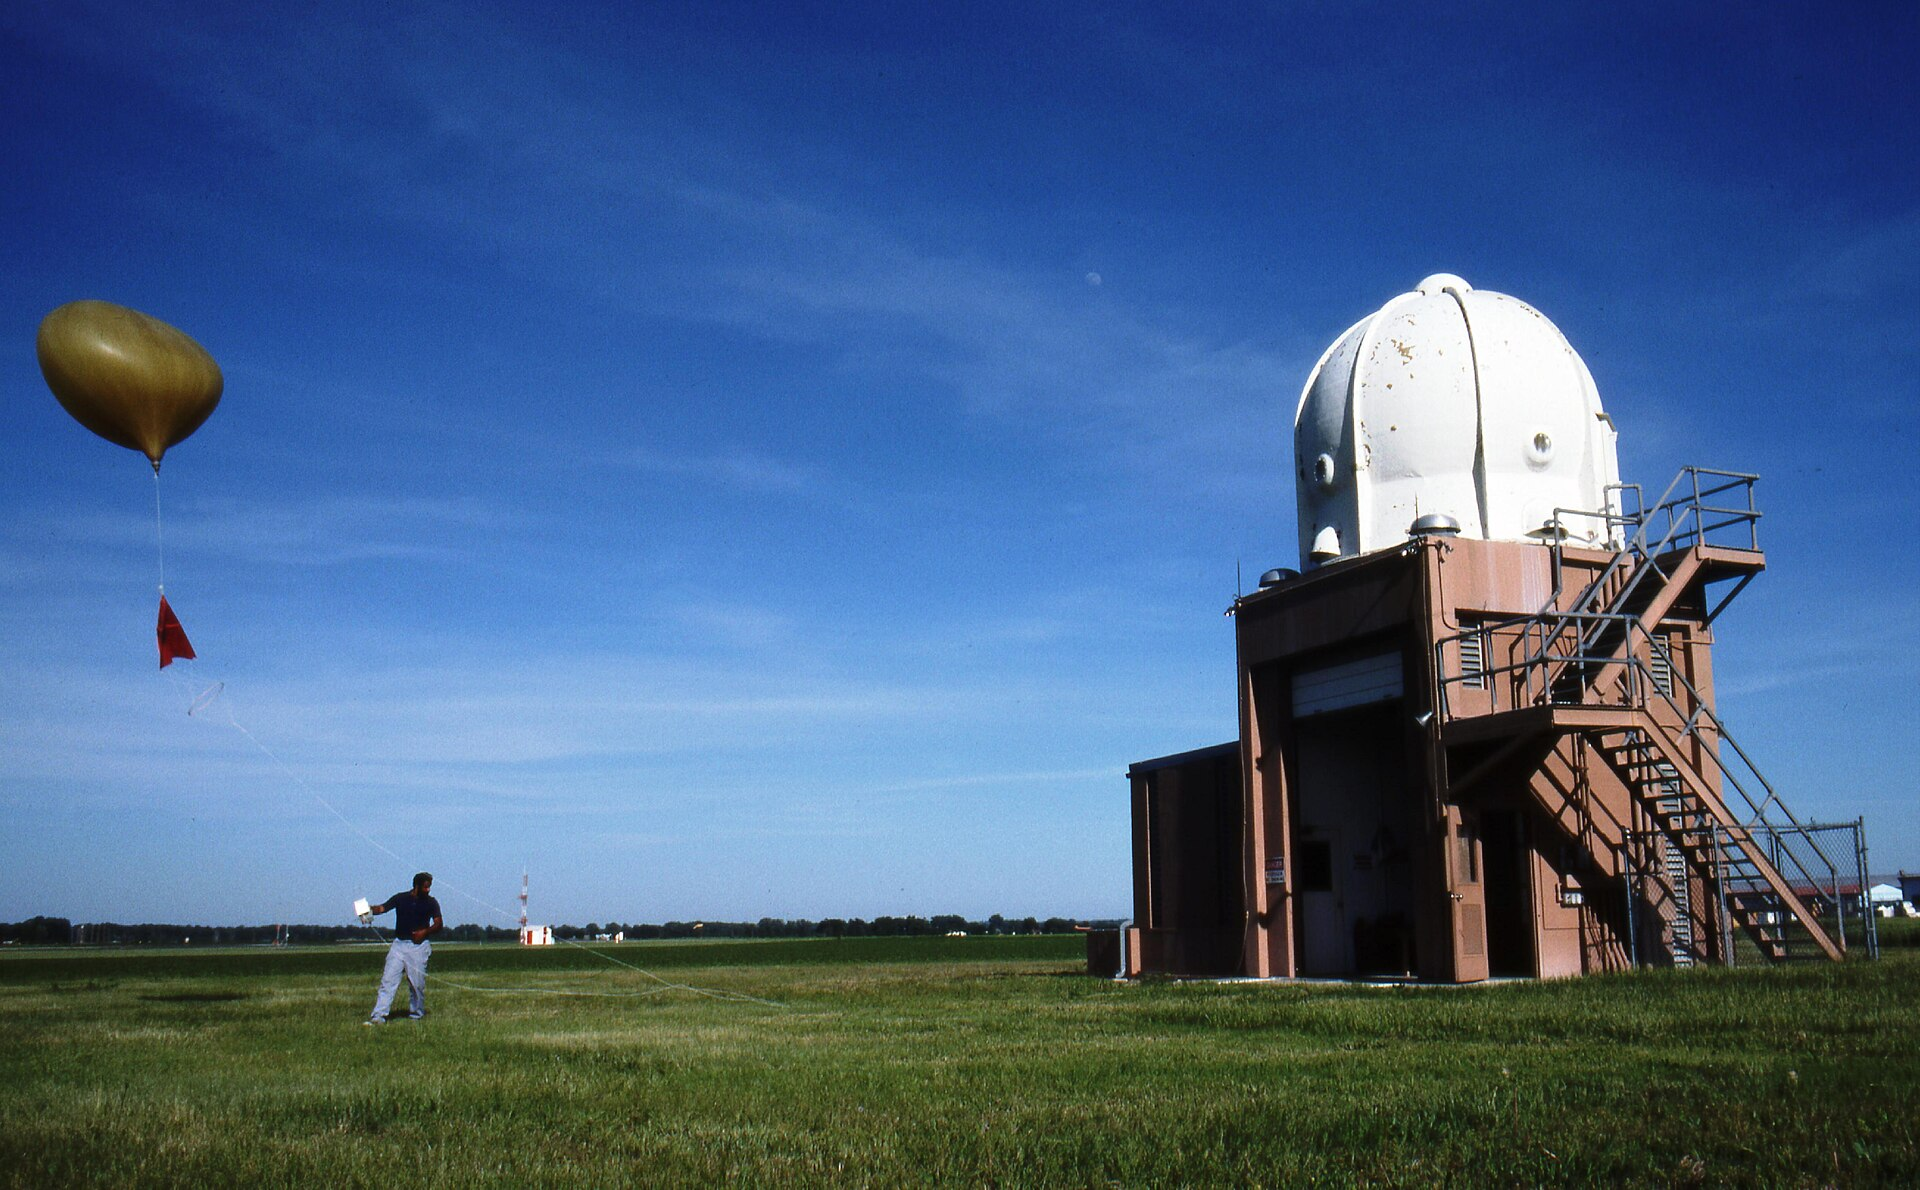
\includegraphics[width=0.78\linewidth]{images/book1/g8-radiosonde-launch.jpg}

{\small Lanzamiento de un globo sonda en Topeka, Kansas (Estados Unidos):
el paracaídas (en rojo) y la radiosonda cuelgan debajo del globo.
Fotografía de Stephen Corfidi, NOAA/National Weather Service (dominio
público, vía Wikimedia Commons).}
% ledger: commons:radiosonde-launch
\label{fig:g8:the-atmosphere:launch}
\end{omfigure}

¿Por qué se hincha el globo a medida que sube? ¿Qué mide la radiosonda
durante la subida, y por qué la temperatura no baja sin más todo el rato?
¿Dónde termina el aire?

\begin{recall}
La \emph{atmósfera} es la capa de aire que rodea la Tierra. El aire
presiona sobre todo lo que toca: es la \emph{presión atmosférica}, que se
mide con un barómetro (los libros de física). Los servicios meteorológicos
la dan en hectopascales (hPa); al \omterm{def:g4:world-physical-map:altitude}{nivel del mar} es de unos
\qty{1013}{hPa}. El aire seco está formado por alrededor de un 78~\% de
nitrógeno y un 21~\% de oxígeno, con un poco de argón, de dióxido de
carbono y de otros gases (los libros de química). Las \omterm{def:g4:clouds-rain-snow:cloud}{nubes} están hechas de
gotitas diminutas de agua o de cristales de hielo (\cref{ch:g4:clouds-rain-snow}).
\end{recall}
% ledger: air:N2, air:O2, ussa76:sea-level

\section{Una envoltura fina}

Vista desde la Estación Espacial Internacional, la atmósfera es una fina
línea luminosa a lo largo del borde de la Tierra. La mayor parte del aire,
y casi todas las \omterm{def:g4:clouds-rain-snow:cloud}{nubes}, están en sus pocos kilómetros más bajos.
% ledger: commons:iss-sunset

\begin{omfigure}
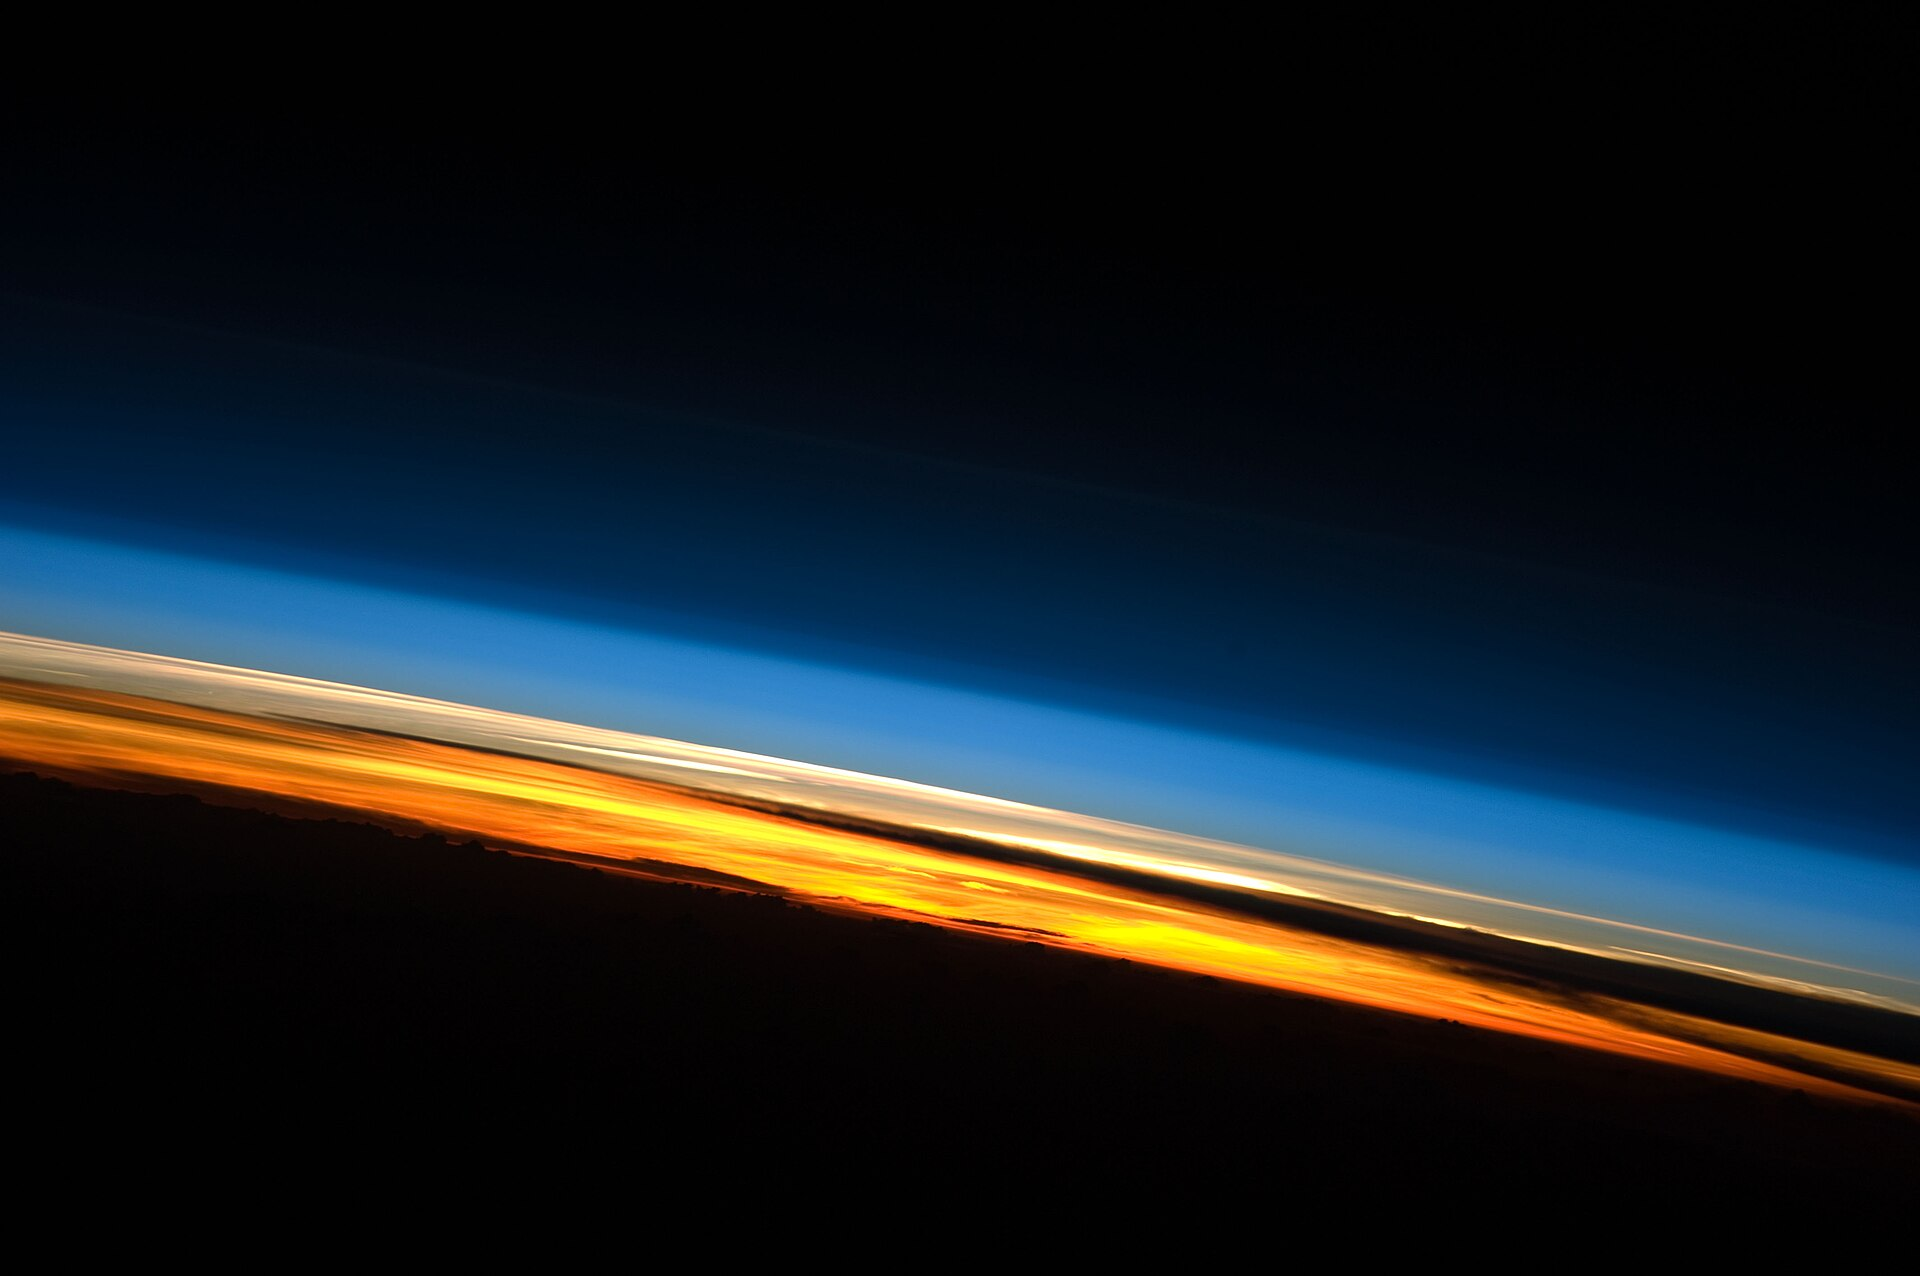
\includegraphics[width=0.78\linewidth]{images/book1/g8-iss-limb.jpg}

{\small El borde de la Tierra a la puesta del sol, fotografiado desde la
Estación Espacial Internacional sobre el \omterm{def:g2:water-on-earth:ocean}{océano} Índico el 14~de junio de
2010. La franja naranja y amarilla es la capa más baja de la atmósfera, con
sus \omterm{def:g4:clouds-rain-snow:cloud}{nubes} oscuras; por encima vienen capas más pálidas y luego azules, que
se funden con el negro del espacio. Fotografía de la NASA, Expedición~23 de
la ISS (dominio público, vía Wikimedia Commons).}
% ledger: commons:iss-sunset
\label{fig:g8:the-atmosphere:limb}
\end{omfigure}

La atmósfera no tiene un techo bien marcado: el aire se va haciendo cada
vez más tenue con la altura. Por convenio, el espacio empieza a unos
\qty{100}{km}. Comparado con el radio de la Tierra, \qty{6371}{km}, es muy
poco: $100 \div
6371 \approx 0.016$, menos del 2~\% del radio. En un \omterm{def:g3:continents-and-oceans:globe}{globo terráqueo} de
\qty{30}{cm} de diámetro, toda la atmósfera sería una película de unos
\qty{2}{mm} de espesor.
% ledger: ucar:layers, earth:Rmean

\begin{omfigure}
\begin{tikzpicture}[font=\footnotesize]
  % 1 cm = 100 km: the Earth's surface is a circle of radius 63.71 cm
  \def\R{63.71}
  \useasboundingbox (-6.9,-1.6) rectangle (6.9,1.0);
  \fill[blue!8] (0,-\R) ++(85:\R+1) arc (85:95:\R+1) -- ($(0,-\R)+(95:\R)$) arc (95:85:\R) -- cycle;
  \fill[omLithAlluv!70] (0,-\R) ++(85:\R) arc (85:95:\R) -- ++(0,-0.6) -- ($(0,-\R)+(85:\R)+(0,-0.6)$) -- cycle;
  \draw[black, line width=0.6pt] (0,-\R) ++(85:\R) arc (85:95:\R);
  \foreach \h/\c in {0.1102/omThm, 0.4938/omMeth, 0.86/omDef} \draw[\c, line width=0.5pt] (0,-\R) ++(85:\R+\h) arc (85:95:\R+\h);
  \draw[black!60, dashed] (0,-\R) ++(85:\R+1) arc (85:95:\R+1);
  \node[anchor=west, omThm] at (5.65,-0.14) {\qty{11}{km}};
  \node[anchor=west, omMeth] at (5.65,0.25) {\qty{49}{km}};
  \node[anchor=west, omDef] at (5.65,0.62) {\qty{86}{km}};
  \node[anchor=east, black!70] at (-5.65,0.75) {\qty{100}{km}};
  \node[anchor=north] at (0,-0.15) {la superficie de la Tierra};
  \draw[|-|] (-5,-1.05) -- node[below] {\qty{1000}{km}} (5,-1.05);
\end{tikzpicture}

{\small Una porción de la Tierra y de su atmósfera dibujada a escala
(\qty{1}{cm} por cada \qty{100}{km}), hasta \qty{100}{km}, el borde del
espacio (línea discontinua). Las líneas de colores son los límites de las
capas que veremos más adelante en este capítulo; la capa más baja, donde
ocurre todo el \omterm{def:g1:watching-the-weather:weather}{tiempo} meteorológico, apenas tiene un milímetro de espesor.}
% ledger: earth:Rmean, ucar:layers (limits: figdata/grade-8/standard_atmosphere.py main table)
\label{fig:g8:the-atmosphere:to-scale}
\end{omfigure}

\section{La presión disminuye con la altitud}

El aire de la parte baja de la atmósfera soporta el peso de todo el aire
que tiene encima. Cuanto más se sube, menos aire queda por encima, y menor
es la presión. En el modelo estándar de la atmósfera que usan los
meteorólogos y los ingenieros, la presión es de \qty{1013}{hPa} al \omterm{def:g4:world-physical-map:altitude}{nivel
del mar}, la mitad a unos \qty{5.5}{km} y la cuarta parte a unos
\qty{10.3}{km}.
% ledger: ussa76:sea-level, ussa76:layers (figdata/grade-8/standard_atmosphere.py main table: half_km 5.48, quarter_km 10.29)

Como la presión mide el peso del aire que hay encima, el nivel de media
presión es también la altura por debajo de la cual está la mitad de todo
el aire: la mitad de la atmósfera está comprimida en sus \qty{5.5}{km} más
bajos. Por debajo de \qty{11}{km} está alrededor del 78~\% del aire, y por
debajo de \qty{30}{km}, alrededor del 99~\%.
% ledger: (computed: figdata/grade-8/standard_atmosphere.py, share_below_11km 77.7, share_below_30km 98.82)

\begin{omfigure}
\begin{minipage}[t]{0.49\linewidth}\centering
\begin{tikzpicture}
\begin{axis}[width=6.6cm, height=7.6cm, xmin=0, xmax=1100, ymin=0, ymax=30,
  xlabel={presión (hPa)}, ylabel={altitud (km)},
  tick label style={font=\scriptsize}, label style={font=\small},
  xtick={0,250,500,750,1000}, ytick={0,5,10,15,20,25,30}]
  \addplot[dashed, black!60] table {figdata/out/grade-8-standard_atmosphere-guides.dat};
  \addplot[omDef, line width=1.1pt] table[x=p_hPa, y=z_km] {figdata/out/grade-8-standard_atmosphere-pressure.dat};
  \addplot[only marks, mark=*, mark size=1.8pt, omThm] table[x=p_hPa, y=z_km] {figdata/out/grade-8-standard_atmosphere-levels.dat};
  \node[anchor=south west, font=\scriptsize, text=black] at (axis cs:506.6,5.48) {la mitad};
  \node[anchor=south west, font=\scriptsize, text=black] at (axis cs:253.3,10.29) {la cuarta parte};
\end{axis}
\end{tikzpicture}

{\small La presión en función de la \omterm{def:g4:world-physical-map:altitude}{altitud}. La presión es la mitad de su
valor al \omterm{def:g4:world-physical-map:altitude}{nivel del mar} a unos \qty{5.5}{km}, y la cuarta parte a unos
\qty{10.3}{km}.}
\end{minipage}\hfill
\begin{minipage}[t]{0.49\linewidth}\centering
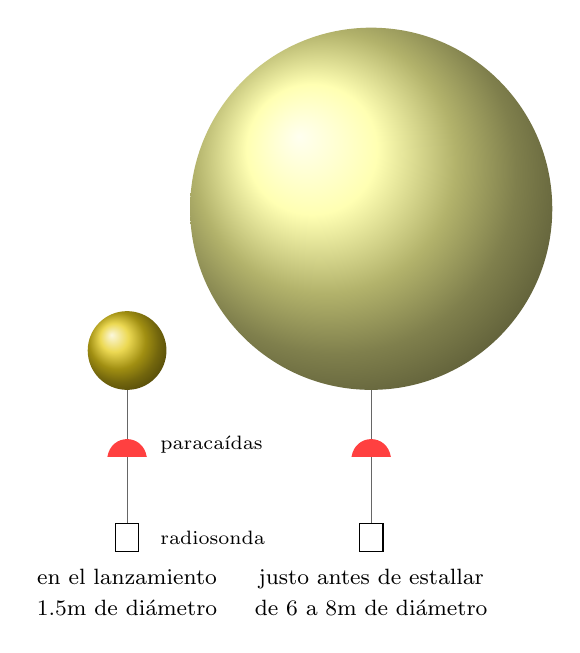
\begin{tikzpicture}[font=\footnotesize]
  % at launch: 1.5 m; at burst: about 7 m (drawn 1 cm for 1.5 m)
  \draw[black!60] (0,0.9) -- (0,2.6);
  \shade[ball color=yellow!60!brown] (0,3.1) circle (0.5);
  \fill[red!75] (-0.25,1.75) .. controls (-0.2,2.05) and (0.2,2.05) .. (0.25,1.75) -- cycle;
  \fill[white, draw=black] (-0.15,0.55) rectangle (0.15,0.9);
  \node[anchor=north] at (0,0.45) {en el lanzamiento};
  \node[anchor=north] at (0,0.05) {\qty{1.5}{m} de diámetro};
  \begin{scope}[xshift=3.1cm]
    \draw[black!60] (0,0.9) -- (0,2.6);
    \shade[ball color=yellow!40!white] (0,4.9) circle (2.3);
    \fill[red!75] (-0.25,1.75) .. controls (-0.2,2.05) and (0.2,2.05) .. (0.25,1.75) -- cycle;
    \fill[white, draw=black] (-0.15,0.55) rectangle (0.15,0.9);
    \node[anchor=north] at (0,0.45) {justo antes de estallar};
    \node[anchor=north] at (0,0.05) {de 6 a \qty{8}{m} de diámetro};
  \end{scope}
  \node[anchor=west, font=\scriptsize] at (0.3,1.9) {paracaídas};
  \node[anchor=west, font=\scriptsize] at (0.3,0.72) {radiosonda};
\end{tikzpicture}

{\small El globo se hincha a medida que sube, porque el aire que lo rodea
presiona cada vez menos (globos y paracaídas a escala entre sí, con la
cuerda acortada).}
% ledger: nws:radiosonde
\end{minipage}
% ledger: ussa76:sea-level, ussa76:layers (figdata/grade-8/standard_atmosphere.py parts pressure, levels, guides)
\label{fig:g8:the-atmosphere:pressure}
\end{omfigure}

Más arriba, la presión sigue bajando, a razón de aproximadamente la mitad
cada pocos kilómetros, así que pronto se vuelve diminuta. Las potencias de
diez son la mejor manera de escribirla. A \qty{30}{km}, la presión es de
unos \qty{12}{hPa}, aproximadamente $10^{-2}$ de su valor al \omterm{def:g4:world-physical-map:altitude}{nivel del mar}
(una centésima); a \qty{50}{km}, de unos \qty{0.8}{hPa}, aproximadamente
$10^{-3}$; a \qty{80}{km}, de unos \qty{0.01}{hPa}, aproximadamente
$10^{-5}$ de la presión al \omterm{def:g4:world-physical-map:altitude}{nivel del mar}.
% ledger: ussa76:layers (figdata/grade-8/standard_atmosphere.py main table: p_30km 11.97, p_50km 0.798, p_80km 0.0105 hPa)

\begin{omfigure}
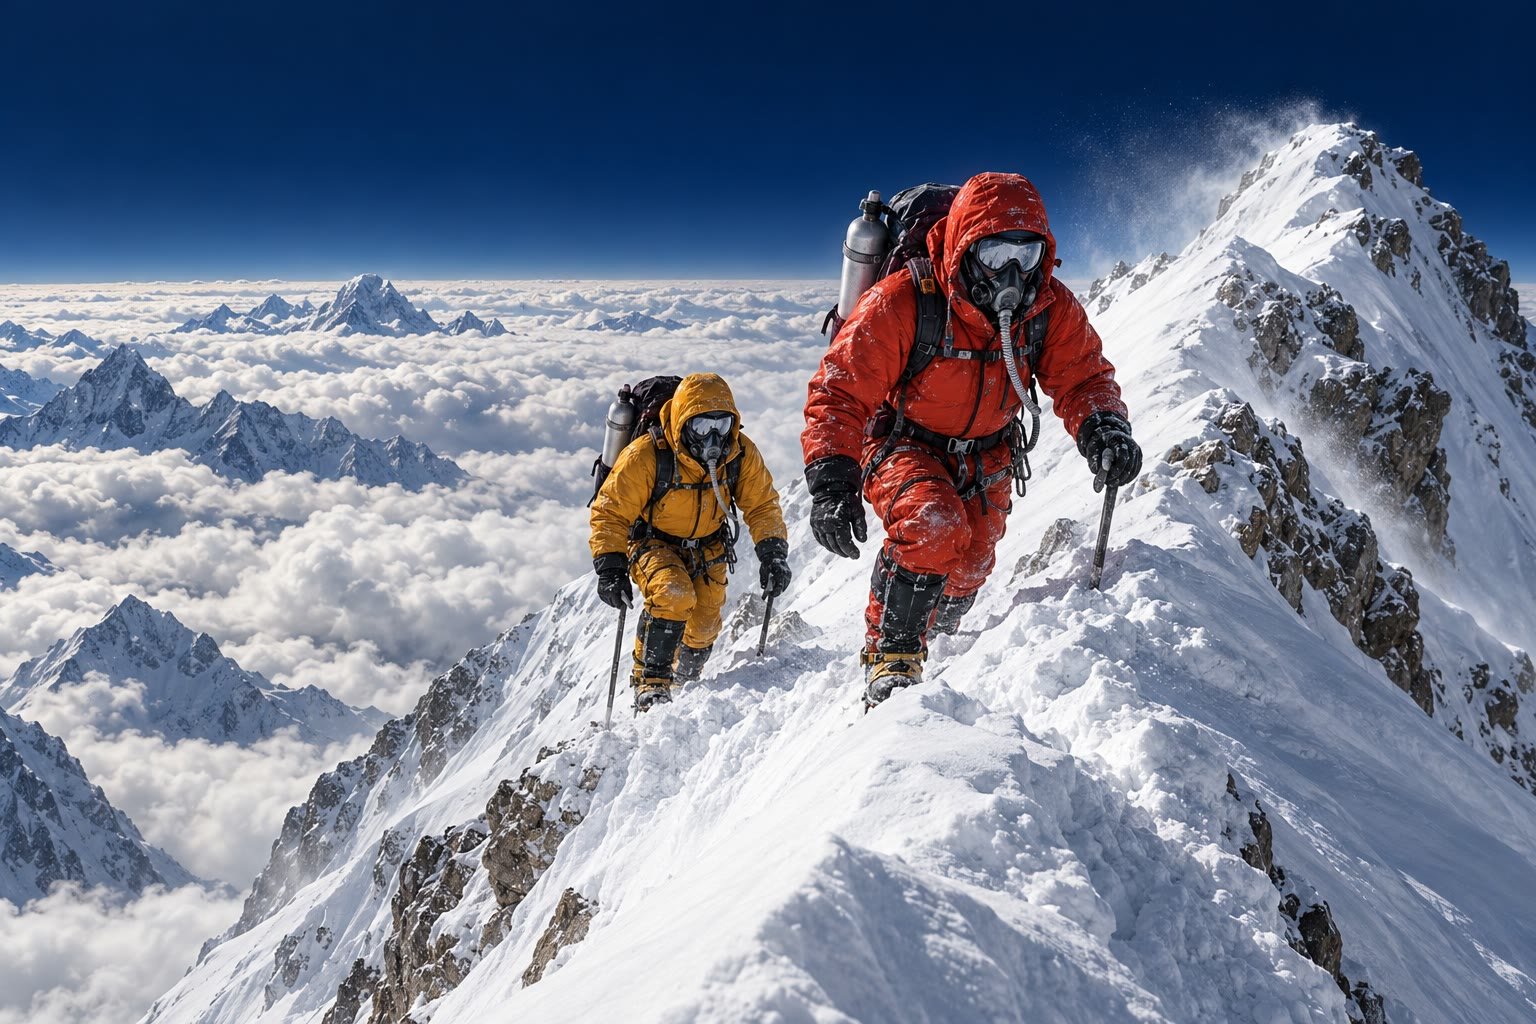
\includegraphics[width=0.5\linewidth]{images/book1/ai/g8-climbers.jpg}

{\small Unos alpinistas en una \omterm{def:g1:landscapes-around-us:landform}{montaña} muy alta llevan botellas de oxígeno.
A \qty{9}{km}, la presión es menos de un tercio de su valor al \omterm{def:g4:world-physical-map:altitude}{nivel del
mar}: el aire sigue conteniendo un 21~\% de oxígeno, pero cada respiración
toma mucho menos (ilustración generada por IA de una escena genérica).}
% ledger: air:O2 (figdata/grade-8/standard_atmosphere.py: pressure at 9 km 308 hPa, 30 % of sea level)
\label{fig:g8:the-atmosphere:climbers}
\end{omfigure}

\section{La temperatura y las capas}

Todo el que ha subido a una \omterm{def:g1:landscapes-around-us:landform}{montaña} sabe que el aire se vuelve más frío con
la altura. Las radiosondas muestran que eso solo es cierto en la parte más
baja de la atmósfera. Más arriba, la temperatura deja de bajar, luego sube,
luego vuelve a bajar y después sube otra vez. Estos cambios dividen la
atmósfera en capas.
% ledger: ucar:layers, ussa76:layers

\begin{omfigure}
\begin{tikzpicture}
\begin{axis}[width=10cm, height=9cm, xmin=-100, xmax=30, ymin=0, ymax=100,
  xlabel={temperatura ($^\circ$C)}, ylabel={altitud (km)},
  tick label style={font=\scriptsize}, label style={font=\small},
  xtick={-100,-80,-60,-40,-20,0,20}, ytick={0,10,20,30,40,50,60,70,80,90,100}, axis on top]
  \addplot[fill=omSea!55, draw=none] table {figdata/out/grade-8-standard_atmosphere-band-troposphere.dat};
  \addplot[fill=omMeth!12, draw=none] table {figdata/out/grade-8-standard_atmosphere-band-stratosphere.dat};
  \addplot[fill=omSea!35, draw=none] table {figdata/out/grade-8-standard_atmosphere-band-mesosphere.dat};
  \addplot[fill=omThm!10, draw=none] table {figdata/out/grade-8-standard_atmosphere-band-thermosphere.dat};
  \addplot[omThm, line width=1.2pt] table[x=T_C, y=z_km] {figdata/out/grade-8-standard_atmosphere-temp.dat};
  \node[anchor=west, font=\small\bfseries, text=black!75] at (axis cs:-97,5.51) {troposfera};
  \node[anchor=west, font=\small\bfseries, text=black!75] at (axis cs:-97,30.2) {estratosfera};
  \node[anchor=west, font=\small\bfseries, text=black!75] at (axis cs:-97,67.69) {mesosfera};
  \node[anchor=west, font=\small\bfseries, text=black!75] at (axis cs:-60,93) {termosfera};
  \draw[black!50, dashed] (axis cs:-100,11.02) -- (axis cs:30,11.02);
  \draw[black!50, dashed] (axis cs:-100,49.38) -- (axis cs:30,49.38);
  \draw[black!50, dashed] (axis cs:-100,86) -- (axis cs:30,86);
  \node[anchor=south east, font=\scriptsize] at (axis cs:17,11.02) {tropopausa};
  \node[anchor=south east, font=\scriptsize] at (axis cs:29,49.38) {estratopausa};
  \node[anchor=south east, font=\scriptsize] at (axis cs:29,86) {mesopausa};
  \fill[omMeth!45] (axis cs:19,16) rectangle (axis cs:23,48);
  \node[anchor=east, font=\scriptsize, align=right] at (axis cs:18,30) {capa\\de ozono};
\end{axis}
\end{tikzpicture}

{\small La temperatura del aire en función de la \omterm{def:g4:world-physical-map:altitude}{altitud}, desde el suelo
hasta \qty{100}{km}, en la atmósfera estándar (una media para las
\omterm{def:g6:latitude-longitude:latitude}{latitudes} medias). Las cuatro capas están sombreadas; la barra verde marca
la altura de la \omterm{def:g8:the-atmosphere:ozone-layer}{capa de ozono}.}
% ledger: ussa76:sea-level, ussa76:layers, ussa76:above-86, ucar:ozone (figdata/grade-8/standard_atmosphere.py parts temp, layers, band-*)
\label{fig:g8:the-atmosphere:temperature}
\end{omfigure}

\begin{definition}[Las capas de la atmósfera]\label{def:g8:the-atmosphere:layers}
De abajo arriba, la atmósfera se divide en cuatro capas según cómo cambia
su temperatura con la altura:
\begin{itemize}
  \item la \emph{troposfera}\index{troposfera}, donde la temperatura
        disminuye con la altura y donde ocurre casi todo el \omterm{def:g1:watching-the-weather:weather}{tiempo}
        meteorológico; su techo es la \emph{tropopausa}\index{tropopausa};
  \item la \emph{estratosfera}\index{estratosfera}, donde la temperatura
        aumenta con la altura, hasta unos \qty{50}{km};
  \item la \emph{mesosfera}\index{mesosfera}, donde la temperatura vuelve
        a disminuir, hasta unos \qty{85}{km};
  \item la \emph{termosfera}\index{termosfera}, donde el aire, muy tenue,
        se calienta cada vez más con la altura.
\end{itemize}
\end{definition}
% ledger: ucar:layers, ussa76:layers

La \omterm{def:g8:the-atmosphere:layers}{troposfera} contiene alrededor del 99~\% del vapor de agua de la
atmósfera, así que casi todas las \omterm{def:g4:clouds-rain-snow:cloud}{nubes}, la \omterm{def:g4:clouds-rain-snow:precipitation}{lluvia} y la \omterm{def:g4:clouds-rain-snow:precipitation}{nieve} se forman en
ella. Su aire se remueve continuamente. El techo de la \omterm{def:g8:the-atmosphere:layers}{troposfera} no está a
la misma altura en todas partes: la \omterm{def:g8:the-atmosphere:layers}{tropopausa} está más alta sobre el
\omterm{def:g3:continents-and-oceans:equator}{ecuador}, donde puede llegar a \qty{20}{km}, y más baja sobre los \omterm{def:g3:continents-and-oceans:poles}{polos},
donde puede bajar hasta \qty{7}{km} en invierno. También está más alta en
verano que en invierno. En la atmósfera estándar, una media para las
\omterm{def:g6:latitude-longitude:latitude}{latitudes} medias, está a \qty{11}{km}.
% ledger: ucar:layers, ucar:tropopause, ussa76:layers

\begin{definition}[Gradiente térmico vertical]\label{def:g8:the-atmosphere:lapse-rate}
El \emph{gradiente térmico vertical}\index{gradiente termico vertical@gradiente térmico vertical}
es el ritmo al que disminuye la temperatura del aire con la altura en la
\omterm{def:g8:the-atmosphere:layers}{troposfera}, en grados Celsius por kilómetro. Cambia de un día a otro y de
un lugar a otro; la atmósfera estándar usa una media de
\qty{6.5}{\degreeCelsius} por kilómetro.
\end{definition}
% ledger: ussa76:layers

\begin{method}[Leer un perfil de temperatura]\label{met:g8:the-atmosphere:profile}
\begin{enumerate}
  \item Busca la \omterm{def:g4:world-physical-map:altitude}{altitud} en el eje vertical y desplázate en horizontal
        hasta la curva; lee la temperatura debajo.
  \item Donde la curva se inclina hacia la izquierda al subir, el aire se
        enfría con la altura; donde se inclina hacia la derecha, el aire se
        calienta con la altura; donde es vertical, la temperatura no cambia.
  \item Los límites entre capas están donde la curva cambia de sentido.
\end{enumerate}
\end{method}

\begin{example}[Un avión de línea a altura de crucero]\label{ex:g8:the-atmosphere:airliner}
Un avión de línea vuela a \qty{11}{km}, cerca de la \omterm{def:g8:the-atmosphere:layers}{tropopausa}. En el
perfil, la temperatura allí es de unos \qty{-56}{\degreeCelsius}. Con el
gradiente térmico: desde \qty{15}{\degreeCelsius} al \omterm{def:g4:world-physical-map:altitude}{nivel del mar}, el aire
se enfría $6.5 \times 11 = 71.5$ grados, lo que da $15 - 71.5 =
\qty{-56.5}{\degreeCelsius}$. En la curva de presión, la presión es de unos
\qty{227}{hPa}, menos de la cuarta parte de la presión en el suelo: la
cabina tiene que estar presurizada.
% ledger: ussa76:sea-level, ussa76:layers (figdata/grade-8/standard_atmosphere.py: T at 11 km -56.4 degC, p 227 hPa)
\end{example}

Por encima de la \omterm{def:g8:the-atmosphere:layers}{tropopausa}, en la \omterm{def:g8:the-atmosphere:layers}{estratosfera}, los aviones de línea
encuentran un vuelo más tranquilo: allí el aire se calienta con la altura,
así que no se remueve desde abajo. En la \omterm{def:g8:the-atmosphere:layers}{mesosfera} se queman la mayoría de
los meteoros, y en su techo, hacia \qty{86}{km}, está el aire más frío de
toda la atmósfera, a unos \qty{-86}{\degreeCelsius}. En la \omterm{def:g8:the-atmosphere:layers}{termosfera}, los
rayos X y la luz ultravioleta del Sol calientan el aire, muy tenue, hasta
cientos, a veces miles, de grados; y sin embargo hay tan poco aire que no
daría sensación de calor. Muchos satélites giran alrededor de la Tierra a
esa altura.
% ledger: ucar:layers, ussa76:above-86

\section{La capa de ozono}

La \omterm{def:g8:the-atmosphere:layers}{estratosfera} se calienta con la altura porque absorbe parte de la luz
del Sol. El gas que hace la mayor parte de este trabajo es el ozono, una
forma del oxígeno (su química está en los libros de química).

\begin{definition}[Capa de ozono]\label{def:g8:the-atmosphere:ozone-layer}
La \emph{capa de ozono}\index{capa de ozono} es la parte de la
\omterm{def:g8:the-atmosphere:layers}{estratosfera}, entre unos \qty{16}{km} y \qty{48}{km}, donde se encuentra
alrededor del 90~\% del ozono de la atmósfera. Absorbe la mayor parte de la
luz ultravioleta perjudicial del Sol.
\end{definition}
% ledger: ucar:ozone

Incluso en la \omterm{def:g8:the-atmosphere:ozone-layer}{capa de ozono}, el ozono es escaso: solo de 1 a 10 moléculas
por cada millón. Y sin embargo, junto con el oxígeno, detiene entre el
95~\% y el 99.9~\% de la luz ultravioleta que llega a la Tierra, incluidas
las clases más perjudiciales. La energía que absorbe se transforma en
calor, y por eso la temperatura aumenta a lo largo de la \omterm{def:g8:the-atmosphere:layers}{estratosfera}. Sin
la \omterm{def:g8:the-atmosphere:ozone-layer}{capa de ozono}, la luz ultravioleta que llegaría al suelo dañaría a los
seres vivos.
% ledger: ucar:ozone

\begin{inthefield}[Seguir los globos sonda]
Los servicios meteorológicos publican las medidas de sus radiosondas, a
menudo como un gráfico de la temperatura en función de la altura para cada
lanzamiento. Con un adulto, busca los sondeos de la estación más cercana,
hechos a las 00:00 o a las 12:00 UTC. Busca la altura a la que la
temperatura deja de bajar: es la \omterm{def:g8:the-atmosphere:layers}{tropopausa} de ese día. Compara un sondeo
de invierno con uno de verano.
\end{inthefield}
% ledger: nws:radiosonde, ucar:tropopause

\section{Ejercicios}

\begin{exercise}[$\star$]\label{exo:g8:the-atmosphere:1}
Une cada capa con su descripción: \omterm{def:g8:the-atmosphere:layers}{troposfera}; \omterm{def:g8:the-atmosphere:layers}{estratosfera}; \omterm{def:g8:the-atmosphere:layers}{mesosfera};
\omterm{def:g8:the-atmosphere:layers}{termosfera}. (a) La temperatura aumenta con la altura y allí se encuentra la
\omterm{def:g8:the-atmosphere:ozone-layer}{capa de ozono}. (b) Allí ocurre casi todo el \omterm{def:g1:watching-the-weather:weather}{tiempo} meteorológico. (c) El
aire más frío de la atmósfera está en su techo. (d) El aire, muy tenue, se
calienta hasta cientos de grados; muchos satélites giran allí.
\end{exercise}

\begin{exercise}[$\star$]\label{exo:g8:the-atmosphere:2}
Usa el perfil de temperatura de la atmósfera estándar. (a) ¿Cuál es la
temperatura al \omterm{def:g4:world-physical-map:altitude}{nivel del mar}? (b) ¿Y a \qty{11}{km}? (c) ¿Y a \qty{50}{km}?
(d) ¿Y a \qty{86}{km}? (e) ¿Entre qué \omterm{def:g4:world-physical-map:altitude}{altitudes} no cambia la temperatura?
\end{exercise}

\begin{exercise}[$\star$]\label{exo:g8:the-atmosphere:3}
¿Verdadero o falso? Corrige las frases falsas. (a) La temperatura del aire
siempre disminuye con la altura. (b) La mitad de todo el aire está por
debajo de unos \qty{5.5}{km}. (c) La \omterm{def:g8:the-atmosphere:ozone-layer}{capa de ozono} está en la \omterm{def:g8:the-atmosphere:layers}{troposfera}.
(d) La \omterm{def:g8:the-atmosphere:layers}{tropopausa} está más alta sobre el \omterm{def:g3:continents-and-oceans:equator}{ecuador} que sobre los \omterm{def:g3:continents-and-oceans:poles}{polos}.
\end{exercise}

\begin{exercise}[$\star$]\label{exo:g8:the-atmosphere:4}
¿En qué capa está cada una de estas cosas? (a) Una \omterm{def:g4:clouds-rain-snow:cloud}{nube} de \omterm{def:g4:clouds-rain-snow:precipitation}{lluvia}. (b) Un
avión de línea a \qty{12}{km}. (c) Un globo sonda justo antes de estallar,
a \qty{32}{km}. (d) Un meteoro que se quema a \qty{75}{km}.
\end{exercise}

\begin{exercise}[$\star\star$]\label{exo:g8:the-atmosphere:5}
Un día de verano hace \qty{20}{\degreeCelsius} al \omterm{def:g4:world-physical-map:altitude}{nivel del mar}. Supón que
el aire se enfría \qty{6.5}{\degreeCelsius} por kilómetro. (a) ¿Qué
temperatura hace a \qty{2}{km}? (b) ¿Y a \qty{3}{km}? (c) ¿A qué altura,
más o menos, llega el aire a \qty{0}{\degreeCelsius}? Redondea a un
decimal.
\end{exercise}

\begin{exercise}[$\star\star$]\label{exo:g8:the-atmosphere:6}
Un refugio de \omterm{def:g1:landscapes-around-us:landform}{montaña} está a \qty{3000}{m}. Un excursionista sale de un
pueblo situado a \qty{500}{m}, donde hace \qty{18}{\degreeCelsius}. Con un
gradiente térmico de \qty{6.5}{\degreeCelsius} por kilómetro: (a) ¿Cuántos
kilómetros sube el excursionista? (b) ¿Cuántos grados se enfría el aire?
(c) ¿Qué temperatura puede esperar en el refugio?
\end{exercise}

\begin{exercise}[$\star\star$]\label{exo:g8:the-atmosphere:7}
Supón que la presión se reduce a la mitad cada \qty{5.5}{km}, partiendo de
\qty{1000}{hPa} al \omterm{def:g4:world-physical-map:altitude}{nivel del mar}. (a) ¿Cuál es la presión a
\qty{5.5}{km}? ¿Y a \qty{11}{km}? ¿Y a \qty{16.5}{km}? (b) La atmósfera
estándar da unos \qty{506}{hPa}, \qty{227}{hPa} y \qty{96}{hPa} a esas tres
alturas (para \qty{1013}{hPa} al \omterm{def:g4:world-physical-map:altitude}{nivel del mar}). ¿Funciona bien la regla de
la mitad cerca del suelo? ¿Y más arriba?
\end{exercise}

\begin{exercise}[$\star\star$]\label{exo:g8:the-atmosphere:8}
Al \omterm{def:g4:world-physical-map:altitude}{nivel del mar}, la presión es de unos \qty{1000}{hPa}, es decir,
$10^3$~hPa. (a) A \qty{30}{km} es de unos \qty{10}{hPa}. Escríbelo como
una potencia de diez y di cuántas veces es menor que al \omterm{def:g4:world-physical-map:altitude}{nivel del mar}.
(b) A \qty{80}{km} es de unos \qty{0.01}{hPa}. Escríbelo como una potencia
de diez. (c) ¿Cuántas veces es menor que al \omterm{def:g4:world-physical-map:altitude}{nivel del mar}?
\end{exercise}

\begin{exercise}[$\star\star$]\label{exo:g8:the-atmosphere:9}
Un globo sonda mide \qty{1.5}{m} de diámetro en el lanzamiento y \qty{6}{m}
cuando estalla. (a) ¿Cuántas veces más ancho es cuando estalla? (b) Explica
por qué se hincha a medida que sube. (c) ¿Por qué los servicios
meteorológicos le cuelgan un paracaídas debajo?
\end{exercise}

\begin{exercise}[$\star\star$]\label{exo:g8:the-atmosphere:10}
La \omterm{def:g8:the-atmosphere:layers}{tropopausa} puede llegar a \qty{20}{km} sobre el \omterm{def:g3:continents-and-oceans:equator}{ecuador} y bajar hasta
\qty{7}{km} sobre los \omterm{def:g3:continents-and-oceans:poles}{polos} en invierno. (a) ¿Cuántas veces más gruesa es,
en ese caso, la \omterm{def:g8:the-atmosphere:layers}{troposfera} sobre el \omterm{def:g3:continents-and-oceans:equator}{ecuador}? Redondea a un decimal. (b) En
el perfil estándar, la \omterm{def:g8:the-atmosphere:layers}{tropopausa} está a \qty{11}{km}. ¿Está la atmósfera
estándar más cerca de la del \omterm{def:g3:continents-and-oceans:equator}{ecuador} o de la de los \omterm{def:g3:continents-and-oceans:poles}{polos}? (c) Un piloto
vuela de una región polar al \omterm{def:g3:continents-and-oceans:equator}{ecuador} a una altura constante de
\qty{10}{km}. ¿Está el avión en la \omterm{def:g8:the-atmosphere:layers}{troposfera} o en la \omterm{def:g8:the-atmosphere:layers}{estratosfera} al
principio (en invierno)? ¿Y al final?
\end{exercise}

\begin{exercise}[$\star\star\star$]\label{exo:g8:the-atmosphere:11}
La parte de todo el aire que está por debajo de una altura es $1 - p \div
p_0$, donde $p$ es la presión a esa altura y $p_0 =
\qty{1013}{hPa}$ la presión al \omterm{def:g4:world-physical-map:altitude}{nivel del mar}. (a) A \qty{5.5}{km}, $p
\approx \qty{506}{hPa}$: ¿qué parte del aire está por debajo? (b) A
\qty{11}{km}, $p \approx \qty{227}{hPa}$. (c) A \qty{30}{km}, $p \approx
\qty{12}{hPa}$. Da las respuestas en tanto por ciento, con números enteros.
(d) ¿Qué parte del aire está por encima de \qty{30}{km}?
\end{exercise}

\begin{exercise}[$\star\star\star$]\label{exo:g8:the-atmosphere:12}
Un \omterm{def:g3:continents-and-oceans:globe}{globo terráqueo} escolar mide \qty{30}{cm} de diámetro, así que su radio,
\qty{15}{cm}, representa el radio de la Tierra, \qty{6371}{km}. (a) ¿Cuántos
kilómetros representa \qty{1}{cm} del \omterm{def:g3:continents-and-oceans:globe}{globo}? Redondea al kilómetro más
cercano. (b) ¿Qué espesor, en milímetros, tendría en este \omterm{def:g3:continents-and-oceans:globe}{globo} la
atmósfera hasta \qty{100}{km}? (c) ¿Y la \omterm{def:g8:the-atmosphere:layers}{troposfera}, de \qty{11}{km} de
espesor? (d) Una hoja de papel tiene unos \qty{0.1}{mm} de espesor.
¿Cuántas hojas formarían la \omterm{def:g8:the-atmosphere:layers}{troposfera} del \omterm{def:g3:continents-and-oceans:globe}{globo}?
\end{exercise}

\section{Problema: seguir un globo sonda}

\begin{problem}[{Problema de fin de semana --- un globo sonda sube a través
de la atmósfera; sus temperaturas muestran las capas, y sus presiones
muestran dónde queda la cuarta parte de la presión al nivel del mar}]
\label{pb:g8:the-atmosphere:1}
% ledger: nws:radiosonde; the table is the standard atmosphere, figdata/grade-8/standard_atmosphere.py part sonde
Se lanza una radiosonda desde una estación situada al \omterm{def:g4:world-physical-map:altitude}{nivel del mar}. Su
globo sube a unos \qty{300}{m} por minuto. La tabla da la presión y la
temperatura que mide (los valores de la atmósfera estándar, redondeados).

\begin{center}\small
\begin{tabular}{|l|*{8}{c|}}
\hline
\omterm{def:g4:world-physical-map:altitude}{altitud} (km) & 0 & 2 & 4 & 6 & 8 & 10 & 12 & 14 \\
\hline
presión (hPa) & 1013 & 795 & 617 & 472 & 357 & 265 & 194 & 142 \\
\hline
temperatura ($^\circ$C) & 15 & 2 & $-11$ & $-24$ & $-37$ & $-50$ & $-56$ & $-56$ \\
\hline
\hline
\omterm{def:g4:world-physical-map:altitude}{altitud} (km) & 16 & 18 & 20 & 22 & 24 & 26 & 28 & 30 \\
\hline
presión (hPa) & 104 & 76 & 55 & 40 & 30 & 22 & 16 & 12 \\
\hline
temperatura ($^\circ$C) & $-56$ & $-56$ & $-56$ & $-55$ & $-53$ & $-51$ & $-49$ & $-47$ \\
\hline
\end{tabular}
\end{center}

\noindent\textbf{Parte I --- La subida.}\par\nopagebreak
\begin{enumerate}[beginpenalty=10000]
  \item ¿Cuántos metros sube el globo en 10 minutos?
  \item ¿Cuánto tarda en llegar a \qty{6}{km}? ¿Y a \qty{30}{km}?
  \item El globo estalla a \qty{30}{km}. ¿Cuánto ha durado el vuelo, en
        horas y minutos?
  \item Di en qué capa está el globo a \qty{8}{km}, y en qué capa está
        cuando estalla.
\end{enumerate}

\noindent\textbf{Parte II --- La temperatura.}\par\nopagebreak
\begin{enumerate}[resume, beginpenalty=10000]
  \item ¿Cuántos grados baja la temperatura entre el suelo y \qty{10}{km}?
  \item ¿Cuál es el gradiente térmico, en grados por kilómetro, en esta
        parte de la subida?
  \item ¿Entre qué \omterm{def:g4:world-physical-map:altitude}{altitudes} se mantiene igual la temperatura? ¿Dónde está
        la \omterm{def:g8:the-atmosphere:layers}{tropopausa}?
  \item ¿Qué le ocurre a la temperatura por encima de \qty{20}{km}? ¿Qué
        gas lo explica?
\end{enumerate}

\noindent\textbf{Parte III --- La presión.}\par\nopagebreak
\begin{enumerate}[resume, beginpenalty=10000]
  \item ¿Cuánto es la mitad de la presión al \omterm{def:g4:world-physical-map:altitude}{nivel del mar}? ¿Entre qué
        \omterm{def:g4:world-physical-map:altitude}{altitudes} se alcanza?
  \item ¿Cuánto es la cuarta parte de la presión al \omterm{def:g4:world-physical-map:altitude}{nivel del mar}? Redondea
        al hectopascal más cercano.
  \item ¿Entre qué dos \omterm{def:g4:world-physical-map:altitude}{altitudes} de la tabla se alcanza esa cuarta parte?
  \item La presión baja \qty{71}{hPa} entre \qty{10}{km} y \qty{12}{km}.
        Suponiendo que baja de manera uniforme, ¿a qué \omterm{def:g4:world-physical-map:altitude}{altitud}, más o menos,
        es la presión la cuarta parte de su valor al \omterm{def:g4:world-physical-map:altitude}{nivel del mar}?
        Redondea a un decimal.
\end{enumerate}
\end{problem}
